% !TEX root =  paper.tex
\section{Preliminary Data Evaluation}
\label{sec:data_eval}
As of writing this paper, there are 654 instances of DigiTaps installed. In addition, we collected 129,906 events which contains 96,892 gesture events. This means that each player performs $\frac{96892}{654} = 148.15$ taps on average. Since there are 3 numbers per level\footnote{DigiTaps has 3 numbers per level until version 1.1.}, the average number of taps per level is $1.8 \times 3 \times 3$, which can be broken down to each digit requires 1.8 taps\footnote{Here we assume that we use Cappuccino method.}, there are 3 digits per number and there 3 numbers per level.

\subsection{Demographics}
The following are the result of the 6 demographics questions we asked.
\begin{enumerate}
  \item \textbf{How old are you?} \\
  47.71\% of the all the players are under the age of 25 (see figure \ref{age}) with players aged between 18 and 25 years old is the largest population in this group. Since DigiTaps is a game, this result is not surprising. People at a younger age may want to try out the game more than the eldery.

\begin{figure}[!htbp]
  \centering
  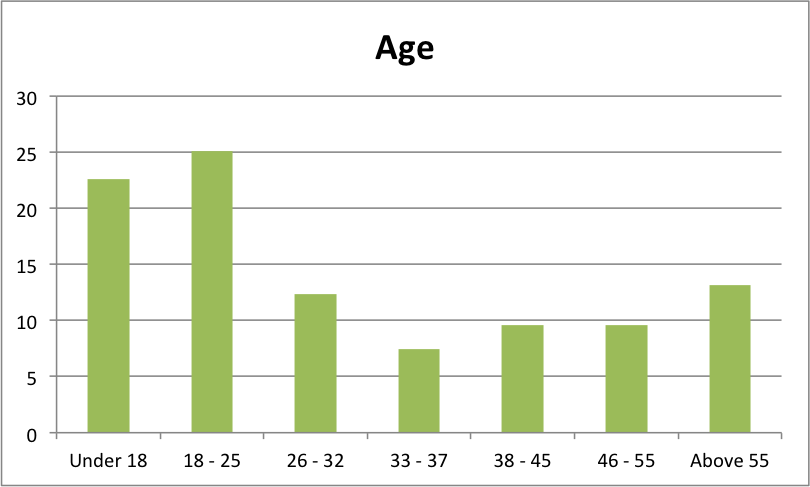
\includegraphics[width=1.0\textwidth]{figures/chart-age.png}
  \caption{This figure shows the breakdown of the age among all the players.}
  \label{age}
  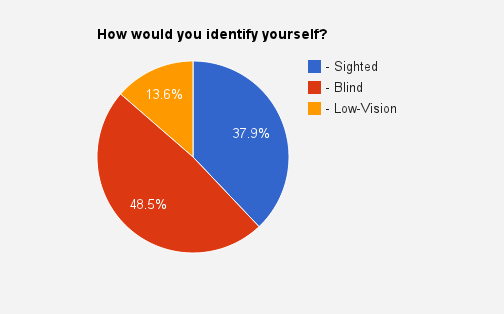
\includegraphics[width=1.0\textwidth]{figures/chart-identity.png}
  \caption{This figure shows the breakdown of players' identification among all the players.}
  \label{identity}
\end{figure}

  \item \textbf{What is your gender?} \\
  The gender are split almost evenly between male and female. Male accounts for 48.01\% and female accounts for 51.99\% of all the DigiTaps players.

  \item \textbf{How would you identify yourself?} \\
  We advertised DigiTaps through several blind organizations' mailing lists. It is not surprising that 48.5\% of the players indentified themselves as blind (see figure \ref{identity}). Sighted players contributes 37.9\% of all the players.

\begin{figure}[!htbp]
  \centering
  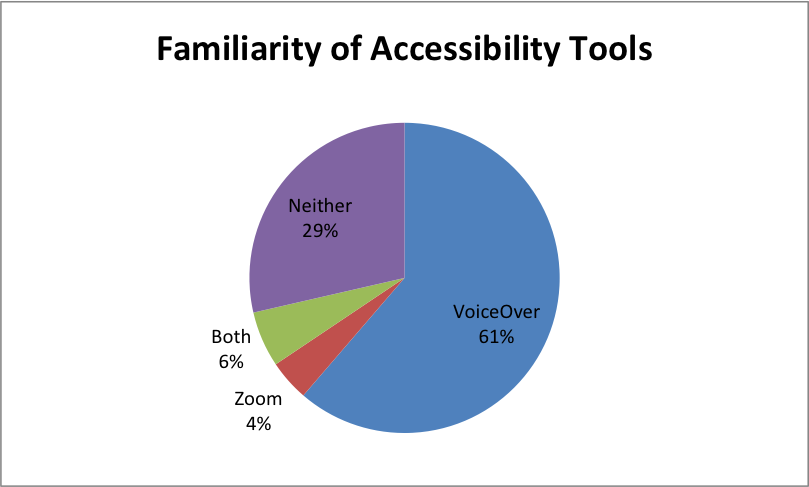
\includegraphics[width=1.0\textwidth]{figures/chart-tools.png}
  \caption{This figure shows the breakdown of the accessibility tool usage among all the players.}
  \label{tool}
  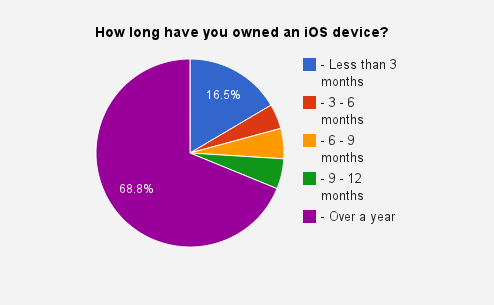
\includegraphics[width=1.0\textwidth]{figures/chart-own.png}
  \caption{This figure shows the breakdown of how long the player possessed his device among all the players.}
  \label{own}
\end{figure}

  \item \textbf{Do you use any accessibility tool on a daily basis?} \\
  Since 48.5\% of the players identified themselves as blind, it is not surprising that the majority of the players uses VoiceOver on a daily basis. However, there are 61.3\% players who use VoiceOver regularly, which is more than 10\% greater than the number of blind players (see figure \ref{tool}. One possible explanation is  13.6\% of the players identified themselves as having low-vision. Low-vision and blind players combined are 62.1\% of all the players.

  \item \textbf{How long have you owned an iOS device?} \\
  Since we only have DigiTaps on iOS, we asked how long that they owned the device, so we can measure their fluency with the platform. The majority, 68.8\%, of the players own their device for over a year (see figure \ref{own}). The second largest population is the players that owns the phone less than 3 months.

\end{enumerate}

\subsection{Touch Events}
Although we have 654 installations of DigiTaps, the number of touch events are too low to do any significant data analysis. There are only 96,892 touch events this is 148.15 touches per user on average. Assuming we are on level 1, which contains 3 3-digit numbers, the whole level requires $2.1 \times 3 \times 3 = 18.9$ taps\footnote{Assuming that we use Espresso method}. Thus, only 7 games were played for each person, which is too low to do in-depth evaluation of the gestures.

Furthermore, we took a closer look into the data using the longitudinal lab study of DigiTaps as the baseline. The study consists of 6 session where each session is divided into 4 conditions. In each condition, the participant is asked to enter 15 random 4-digit numbers \cite{Azenkot:2013}. This gives us $4 \times 15 \times 4 \times 6 = 1,440$ digits total. Assuming we use the Espresso method, the player has to perform $2.1 \times 1,440 = 3,024$ taps on average. Hence, we only consider players that performed more than 3,024 gestures. Looking closer into the data, there are only 6 players that has performed the gestures more than 3,024 times. 6 players is too few to do any in-depth analysis on the data. 
